%% SoftwareX original software publication: Fermium Hazard Mapper.
%% Built on elsarticle, following the SoftwareX template's section order and
%% code metadata table. Every reported value is a macro from ../numbers.tex,
%% which docs/build_numbers.py writes from the pipeline outputs, or from
%% national.tex, which build_national.py writes from the national partition.
%% Build: latexmk -pdf softwarex.tex   (run from docs/softwarex/)

\documentclass[preprint,12pt]{elsarticle}

\usepackage{amssymb}
\usepackage{graphicx}
\usepackage{booktabs}
\usepackage{tabularx}
\usepackage{siunitx}
\usepackage[hidelinks]{hyperref}
\usepackage{xurl}
\usepackage{listings}
\usepackage{float}
\usepackage{xcolor}

% Code, file names, URLs and the command listing use the body font, not a
% typewriter face, so the text reads in one typeface throughout.
\renewcommand{\ttdefault}{\rmdefault}
\urlstyle{same}

\lstset{basicstyle=\footnotesize\ttfamily, breaklines=true,
        columns=fullflexible, frame=tb, framerule=0.3pt}

\graphicspath{{../}}
% Generated by docs/build_numbers.py — do not edit by hand.
% Built 2026-09-29T15:16:37+00:00
%
% Any figure the pipeline did not produce renders as \todo{missing},
% so a gap is visible in the PDF rather than filled from memory.
\providecommand{\todo}[1]{\textbf{[TODO: #1]}}

% ---- rangpur_rajshahi ----
\newcommand{\RRAssets}{23,016}
\newcommand{\RRMappedCellShare}{12.5}
\newcommand{\RRLabelRate}{6.7}
\newcommand{\RRValAUC}{0.884}
\newcommand{\RRValAP}{0.234}
\newcommand{\RRValAPLift}{7.032}
\newcommand{\RRValBrier}{0.069}
\newcommand{\RRValBrierCalibrated}{0.029}
\newcommand{\RRValBrierBaseRate}{0.032}
\newcommand{\RRNCalibration}{1,474}
\newcommand{\RRNTrain}{18,687}
\newcommand{\RRNVal}{2,855}
\newcommand{\RRScoreMean}{0.068}
\newcommand{\RRScoreMedian}{0.013}
\newcommand{\RRKrigingVar}{0.037}
\newcommand{\RRKrigingSillRatio}{0.442}
\newcommand{\RRVariogramRange}{1.087}
\newcommand{\RRNuggetSillRatio}{0.307}
\newcommand{\RRProcessed}{2026-09-29}
\newcommand{\RRNVulnComponents}{4}
\newcommand{\RRObsEvents}{5}
\newcommand{\RRObsFloodedShare}{6.7}
\newcommand{\RRObsAUC}{0.879}
\newcommand{\RRObsAPLift}{6.307}
\newcommand{\RRObsBrierCalibrated}{0.03}
\newcommand{\RRProxyPOD}{0.151}
\newcommand{\RRProxyFAR}{0.517}
\newcommand{\RRProxyCSI}{0.13}
\newcommand{\RRProxyKappa}{0.144}
\newcommand{\RRProxyShare}{6.6}
\newcommand{\RRObservedShare}{21.2}
\newcommand{\RRMinEvents}{2}
\newcommand{\RRSurfaceKrigedObsAUC}{0.666}
\newcommand{\RRSurfaceTerrainObsAUC}{0.657}
\newcommand{\RRProxyTrainedObsAUC}{0.809}
\newcommand{\RRProxyTrainedObsAPLift}{2.382}
\newcommand{\RRCalibBlockRate}{6.4}
\newcommand{\RRTestBlockRate}{3.3}
\newcommand{\RRKrigedGridSD}{0.13}
\newcommand{\RRTerrainGridSD}{0.24}
\newcommand{\RRHazardAUC}{0.621}
\newcommand{\RRHazardAP}{0.08}
\newcommand{\RRHazCoefElevation}{-0.811}
\newcommand{\RRHazCoefSlope}{0.027}
\newcommand{\RRHazCoefTwi}{0.064}
\newcommand{\RRHazCoefHand}{-0.032}
\newcommand{\RRHazCoefFlowAcc}{-0.021}
\newcommand{\RRBenchGraphAUC}{0.789}
\newcommand{\RRBenchGraphSD}{0.047}
\newcommand{\RRBenchGraphLift}{3.57}
\newcommand{\RRBenchLogisticAUC}{0.786}
\newcommand{\RRBenchLogisticSD}{0.039}
\newcommand{\RRBenchLogisticLift}{3.28}
\newcommand{\RRBenchForestAUC}{0.816}
\newcommand{\RRBenchForestSD}{0.044}
\newcommand{\RRBenchForestLift}{4.65}
\newcommand{\RRBenchBoostingAUC}{0.817}
\newcommand{\RRBenchBoostingSD}{0.045}
\newcommand{\RRBenchBoostingLift}{4.21}
\newcommand{\RRBenchTwiAUC}{0.517}
\newcommand{\RRBenchTwiSD}{0.03}
\newcommand{\RRBenchTwiLift}{1.24}
\newcommand{\RRBenchBest}{gradient boosting}
\newcommand{\RRBenchDiff}{-0.028}
\newcommand{\RRBenchGap}{0.028}
\newcommand{\RRBenchDiffP}{<0.001}
\newcommand{\RRBenchAhead}{2}
\newcommand{\RRBenchSeeds}{20}
\newcommand{\RRLabelObsAUC}{0.817}
\newcommand{\RRLabelObsSD}{0.045}
\newcommand{\RRLabelProxyAUC}{0.716}
\newcommand{\RRLabelProxySD}{0.055}
\newcommand{\RRLabelGap}{0.101}
\newcommand{\RRLabelGapP}{<0.001}
\newcommand{\RRLabelAhead}{20}
\newcommand{\RRTempAUC}{0.801}
\newcommand{\RRTempSD}{0.063}
\newcommand{\RRTempLift}{6.354}
\newcommand{\RRTempAllAUC}{0.794}
\newcommand{\RRTempPastAUC}{0.896}
\newcommand{\RRTempPastSD}{0.042}
\newcommand{\RRTempPastLift}{21.717}
\newcommand{\RRTempMinusPast}{-0.094}
\newcommand{\RRTempMinusPastP}{<0.001}
\newcommand{\RRTempAheadPast}{2}
\newcommand{\RRTempMinusAll}{0.008}
\newcommand{\RRTempMinusAllP}{=0.052}
\newcommand{\RRTempPastGap}{0.094}
\newcommand{\RRTempAllGap}{0.008}
\newcommand{\RRTempSeeds}{20}
\newcommand{\RRTempTestRate}{2.8}
\newcommand{\RRTempProxyAUC}{0.732}
\newcommand{\RRTempProxySD}{0.067}
\newcommand{\RRTempProxyGap}{0.069}
\newcommand{\RRTempProxyGapP}{<0.001}
\newcommand{\RRTempProxyAhead}{18}
\newcommand{\RRXcCells}{645,527}
\newcommand{\RRXcSOneShare}{19.7}
\newcommand{\RRXcGfdShare}{13.2}
\newcommand{\RRXcPOD}{0.559}
\newcommand{\RRXcFAR}{0.624}
\newcommand{\RRXcCSI}{0.29}
\newcommand{\RRXcKappa}{0.346}
\newcommand{\RRXcAgree}{81.9}
\newcommand{\RRXcAUC}{0.783}
\newcommand{\RRImpElevation}{0.086}
\newcommand{\RRImpOtherTerrainMax}{0}
\newcommand{\RRImpTerrain}{0.08}
\newcommand{\RRImpAccess}{0.11}
\newcommand{\RRImpPopulation}{0.081}
\newcommand{\RRImpAssetType}{0.043}
\newcommand{\RRPastFeatAUC}{0.924}
\newcommand{\RRPastFeatSD}{0.035}
\newcommand{\RRPastFeatWithoutAUC}{0.79}
\newcommand{\RRPastFeatOnlyAUC}{0.896}
\newcommand{\RRPastFeatOverPast}{0.029}
\newcommand{\RRPastFeatOverPastP}{<0.001}
\newcommand{\RRPastFeatOverPastAhead}{16}
\newcommand{\RRPastFeatOverWithout}{0.134}
\newcommand{\RRPastFeatOverWithoutP}{<0.001}
\newcommand{\RRPastFeatUnseenAUC}{0.729}
\newcommand{\RRPastFeatUnseenShare}{87.7}
\newcommand{\RRPastFeatUnseenPos}{16.9}
\newcommand{\RRSensEqualTypesRho}{0.942}
\newcommand{\RRSensPopOnlyRho}{0.663}
\newcommand{\RRSensExposureDoubleRho}{0.946}
\newcommand{\RRSensExposureDoubleTop}{0.829}
\newcommand{\RRSensRandomRho}{0.963}
\newcommand{\RRSensRandomRhoMin}{0.914}
\newcommand{\RRSensRandomTop}{0.87}
\newcommand{\RRSensDraws}{20}
\newcommand{\RRNUnions}{1,339}
\newcommand{\RRNUnionsScored}{1,199}
\newcommand{\RRNUpazilas}{148}
\newcommand{\RRNUpazilasScored}{147}
\newcommand{\RRNDistricts}{21}
\newcommand{\RRNDistrictsScored}{21}

% ---- sylhet ----
\newcommand{\SylhetAssets}{13,374}
\newcommand{\SylhetMappedCellShare}{10.3}
\newcommand{\SylhetLabelRate}{14.7}
\newcommand{\SylhetValAUC}{0.934}
\newcommand{\SylhetValAP}{0.639}
\newcommand{\SylhetValAPLift}{6.062}
\newcommand{\SylhetValBrier}{0.073}
\newcommand{\SylhetValBrierCalibrated}{0.057}
\newcommand{\SylhetValBrierBaseRate}{0.094}
\newcommand{\SylhetNCalibration}{953}
\newcommand{\SylhetNTrain}{11,026}
\newcommand{\SylhetNVal}{1,395}
\newcommand{\SylhetScoreMean}{0.274}
\newcommand{\SylhetScoreMedian}{0.079}
\newcommand{\SylhetKrigingVar}{0.095}
\newcommand{\SylhetKrigingSillRatio}{0.933}
\newcommand{\SylhetVariogramRange}{0.136}
\newcommand{\SylhetNuggetSillRatio}{0.742}
\newcommand{\SylhetProcessed}{2026-09-29}
\newcommand{\SylhetNVulnComponents}{4}
\newcommand{\SylhetObsEvents}{4}
\newcommand{\SylhetObsFloodedShare}{14.7}
\newcommand{\SylhetObsAUC}{0.934}
\newcommand{\SylhetObsAPLift}{5.957}
\newcommand{\SylhetObsBrierCalibrated}{0.057}
\newcommand{\SylhetProxyPOD}{0.273}
\newcommand{\SylhetProxyFAR}{0.626}
\newcommand{\SylhetProxyCSI}{0.187}
\newcommand{\SylhetProxyKappa}{0.176}
\newcommand{\SylhetProxyShare}{14.7}
\newcommand{\SylhetObservedShare}{20.1}
\newcommand{\SylhetMinEvents}{2}
\newcommand{\SylhetSurfaceKrigedObsAUC}{0.544}
\newcommand{\SylhetSurfaceTerrainObsAUC}{0.822}
\newcommand{\SylhetProxyTrainedObsAUC}{0.847}
\newcommand{\SylhetProxyTrainedObsAPLift}{3.275}
\newcommand{\SylhetCalibBlockRate}{13.7}
\newcommand{\SylhetTestBlockRate}{10.5}
\newcommand{\SylhetKrigedGridSD}{0.11}
\newcommand{\SylhetTerrainGridSD}{0.26}
\newcommand{\SylhetHazardAUC}{0.788}
\newcommand{\SylhetHazardAP}{0.263}
\newcommand{\SylhetHazCoefElevation}{-1.264}
\newcommand{\SylhetHazCoefSlope}{-0.244}
\newcommand{\SylhetHazCoefTwi}{-0.102}
\newcommand{\SylhetHazCoefHand}{0.033}
\newcommand{\SylhetHazCoefFlowAcc}{-0.227}
\newcommand{\SylhetBenchGraphAUC}{0.854}
\newcommand{\SylhetBenchGraphSD}{0.039}
\newcommand{\SylhetBenchGraphLift}{3.84}
\newcommand{\SylhetBenchLogisticAUC}{0.855}
\newcommand{\SylhetBenchLogisticSD}{0.036}
\newcommand{\SylhetBenchLogisticLift}{3.4}
\newcommand{\SylhetBenchForestAUC}{0.845}
\newcommand{\SylhetBenchForestSD}{0.052}
\newcommand{\SylhetBenchForestLift}{3.76}
\newcommand{\SylhetBenchBoostingAUC}{0.857}
\newcommand{\SylhetBenchBoostingSD}{0.042}
\newcommand{\SylhetBenchBoostingLift}{3.9}
\newcommand{\SylhetBenchTwiAUC}{0.535}
\newcommand{\SylhetBenchTwiSD}{0.029}
\newcommand{\SylhetBenchTwiLift}{1.14}
\newcommand{\SylhetBenchBest}{gradient boosting}
\newcommand{\SylhetBenchDiff}{-0.003}
\newcommand{\SylhetBenchGap}{0.003}
\newcommand{\SylhetBenchDiffP}{=0.674}
\newcommand{\SylhetBenchAhead}{7}
\newcommand{\SylhetBenchSeeds}{20}
\newcommand{\SylhetLabelObsAUC}{0.857}
\newcommand{\SylhetLabelObsSD}{0.042}
\newcommand{\SylhetLabelProxyAUC}{0.77}
\newcommand{\SylhetLabelProxySD}{0.048}
\newcommand{\SylhetLabelGap}{0.087}
\newcommand{\SylhetLabelGapP}{<0.001}
\newcommand{\SylhetLabelAhead}{19}
\newcommand{\SylhetTempAUC}{0.797}
\newcommand{\SylhetTempSD}{0.064}
\newcommand{\SylhetTempLift}{2.989}
\newcommand{\SylhetTempAllAUC}{0.85}
\newcommand{\SylhetTempPastAUC}{0.851}
\newcommand{\SylhetTempPastSD}{0.039}
\newcommand{\SylhetTempPastLift}{3.822}
\newcommand{\SylhetTempMinusPast}{-0.054}
\newcommand{\SylhetTempMinusPastP}{<0.001}
\newcommand{\SylhetTempAheadPast}{4}
\newcommand{\SylhetTempMinusAll}{-0.053}
\newcommand{\SylhetTempMinusAllP}{<0.001}
\newcommand{\SylhetTempPastGap}{0.054}
\newcommand{\SylhetTempAllGap}{0.053}
\newcommand{\SylhetTempSeeds}{20}
\newcommand{\SylhetTempTestRate}{17.7}
\newcommand{\SylhetTempProxyAUC}{0.773}
\newcommand{\SylhetTempProxySD}{0.043}
\newcommand{\SylhetTempProxyGap}{0.024}
\newcommand{\SylhetTempProxyGapP}{=0.063}
\newcommand{\SylhetTempProxyAhead}{15}
\newcommand{\SylhetXcCells}{342,128}
\newcommand{\SylhetXcSOneShare}{13.2}
\newcommand{\SylhetXcGfdShare}{23.3}
\newcommand{\SylhetXcPOD}{0.396}
\newcommand{\SylhetXcFAR}{0.3}
\newcommand{\SylhetXcCSI}{0.339}
\newcommand{\SylhetXcKappa}{0.406}
\newcommand{\SylhetXcAgree}{82}
\newcommand{\SylhetXcAUC}{0.746}
\newcommand{\SylhetImpElevation}{0.22}
\newcommand{\SylhetImpOtherTerrainMax}{0.009}
\newcommand{\SylhetImpTerrain}{0.214}
\newcommand{\SylhetImpAccess}{0.133}
\newcommand{\SylhetImpPopulation}{0.032}
\newcommand{\SylhetImpAssetType}{0.02}
\newcommand{\SylhetPastFeatAUC}{0.849}
\newcommand{\SylhetPastFeatSD}{0.046}
\newcommand{\SylhetPastFeatWithoutAUC}{0.837}
\newcommand{\SylhetPastFeatOnlyAUC}{0.851}
\newcommand{\SylhetPastFeatOverPast}{-0.002}
\newcommand{\SylhetPastFeatOverPastP}{=0.767}
\newcommand{\SylhetPastFeatOverPastAhead}{9}
\newcommand{\SylhetPastFeatOverWithout}{0.011}
\newcommand{\SylhetPastFeatOverWithoutP}{=0.015}
\newcommand{\SylhetPastFeatUnseenAUC}{0.777}
\newcommand{\SylhetPastFeatUnseenShare}{79.8}
\newcommand{\SylhetPastFeatUnseenPos}{22.3}
\newcommand{\SylhetSensEqualTypesRho}{0.901}
\newcommand{\SylhetSensPopOnlyRho}{0.431}
\newcommand{\SylhetSensExposureDoubleRho}{0.952}
\newcommand{\SylhetSensExposureDoubleTop}{0.779}
\newcommand{\SylhetSensRandomRho}{0.956}
\newcommand{\SylhetSensRandomRhoMin}{0.913}
\newcommand{\SylhetSensRandomTop}{0.802}
\newcommand{\SylhetSensDraws}{20}
\newcommand{\SylhetNUnions}{717}
\newcommand{\SylhetNUnionsScored}{642}
\newcommand{\SylhetNUpazilas}{78}
\newcommand{\SylhetNUpazilasScored}{78}
\newcommand{\SylhetNDistricts}{10}
\newcommand{\SylhetNDistrictsScored}{10}

% ---- sw_coastal ----
\newcommand{\CoastalAssets}{29,545}
\newcommand{\CoastalMappedCellShare}{11.6}
\newcommand{\CoastalLabelRate}{4.5}
\newcommand{\CoastalValAUC}{0.794}
\newcommand{\CoastalValAP}{0.044}
\newcommand{\CoastalValAPLift}{2.544}
\newcommand{\CoastalValBrier}{0.134}
\newcommand{\CoastalValBrierCalibrated}{0.039}
\newcommand{\CoastalValBrierBaseRate}{0.017}
\newcommand{\CoastalNCalibration}{2,472}
\newcommand{\CoastalNTrain}{23,635}
\newcommand{\CoastalNVal}{3,438}
\newcommand{\CoastalScoreMean}{0.226}
\newcommand{\CoastalScoreMedian}{0.084}
\newcommand{\CoastalKrigingVar}{0.064}
\newcommand{\CoastalKrigingSillRatio}{0.844}
\newcommand{\CoastalVariogramRange}{0.289}
\newcommand{\CoastalNuggetSillRatio}{0.702}
\newcommand{\CoastalProcessed}{2026-09-29}
\newcommand{\CoastalNVulnComponents}{4}
\newcommand{\CoastalObsEvents}{4}
\newcommand{\CoastalObsFloodedShare}{4.4}
\newcommand{\CoastalObsAUC}{0.786}
\newcommand{\CoastalObsAPLift}{2.444}
\newcommand{\CoastalObsBrierCalibrated}{0.039}
\newcommand{\CoastalProxyPOD}{0.224}
\newcommand{\CoastalProxyFAR}{0.956}
\newcommand{\CoastalProxyCSI}{0.039}
\newcommand{\CoastalProxyKappa}{0.037}
\newcommand{\CoastalProxyShare}{11.8}
\newcommand{\CoastalObservedShare}{2.3}
\newcommand{\CoastalMinEvents}{1}
\newcommand{\CoastalSurfaceKrigedObsAUC}{0.538}
\newcommand{\CoastalSurfaceTerrainObsAUC}{0.542}
\newcommand{\CoastalProxyTrainedObsAUC}{0.814}
\newcommand{\CoastalProxyTrainedObsAPLift}{3.374}
\newcommand{\CoastalCalibBlockRate}{5.5}
\newcommand{\CoastalTestBlockRate}{1.7}
\newcommand{\CoastalKrigedGridSD}{0.13}
\newcommand{\CoastalTerrainGridSD}{0.38}
\newcommand{\CoastalHazardAUC}{0.757}
\newcommand{\CoastalHazardAP}{0.062}
\newcommand{\CoastalHazCoefElevation}{-1.166}
\newcommand{\CoastalHazCoefSlope}{-0.59}
\newcommand{\CoastalHazCoefTwi}{-0.27}
\newcommand{\CoastalHazCoefHand}{0.107}
\newcommand{\CoastalHazCoefFlowAcc}{-0.193}
\newcommand{\CoastalBenchGraphAUC}{0.817}
\newcommand{\CoastalBenchGraphSD}{0.057}
\newcommand{\CoastalBenchGraphLift}{4.11}
\newcommand{\CoastalBenchLogisticAUC}{0.809}
\newcommand{\CoastalBenchLogisticSD}{0.046}
\newcommand{\CoastalBenchLogisticLift}{3.07}
\newcommand{\CoastalBenchForestAUC}{0.838}
\newcommand{\CoastalBenchForestSD}{0.049}
\newcommand{\CoastalBenchForestLift}{5}
\newcommand{\CoastalBenchBoostingAUC}{0.839}
\newcommand{\CoastalBenchBoostingSD}{0.046}
\newcommand{\CoastalBenchBoostingLift}{4.51}
\newcommand{\CoastalBenchTwiAUC}{0.577}
\newcommand{\CoastalBenchTwiSD}{0.041}
\newcommand{\CoastalBenchTwiLift}{1.32}
\newcommand{\CoastalBenchBest}{gradient boosting}
\newcommand{\CoastalBenchDiff}{-0.022}
\newcommand{\CoastalBenchGap}{0.022}
\newcommand{\CoastalBenchDiffP}{=0.04}
\newcommand{\CoastalBenchAhead}{6}
\newcommand{\CoastalBenchSeeds}{20}
\newcommand{\CoastalLabelObsAUC}{0.839}
\newcommand{\CoastalLabelObsSD}{0.046}
\newcommand{\CoastalLabelProxyAUC}{0.758}
\newcommand{\CoastalLabelProxySD}{0.053}
\newcommand{\CoastalLabelGap}{0.08}
\newcommand{\CoastalLabelGapP}{<0.001}
\newcommand{\CoastalLabelAhead}{19}
\newcommand{\CoastalTempAUC}{0.807}
\newcommand{\CoastalTempSD}{0.055}
\newcommand{\CoastalTempLift}{5.297}
\newcommand{\CoastalTempAllAUC}{0.834}
\newcommand{\CoastalTempPastAUC}{0.668}
\newcommand{\CoastalTempPastSD}{0.072}
\newcommand{\CoastalTempPastLift}{10.922}
\newcommand{\CoastalTempMinusPast}{0.138}
\newcommand{\CoastalTempMinusPastP}{<0.001}
\newcommand{\CoastalTempAheadPast}{19}
\newcommand{\CoastalTempMinusAll}{-0.028}
\newcommand{\CoastalTempMinusAllP}{=0.001}
\newcommand{\CoastalTempPastGap}{0.138}
\newcommand{\CoastalTempAllGap}{0.028}
\newcommand{\CoastalTempSeeds}{20}
\newcommand{\CoastalTempTestRate}{2.9}
\newcommand{\CoastalTempProxyAUC}{0.736}
\newcommand{\CoastalTempProxySD}{0.066}
\newcommand{\CoastalTempProxyGap}{0.071}
\newcommand{\CoastalTempProxyGapP}{<0.001}
\newcommand{\CoastalTempProxyAhead}{18}
\newcommand{\CoastalXcCells}{\todo{missing}}
\newcommand{\CoastalXcSOneShare}{\todo{missing}}
\newcommand{\CoastalXcGfdShare}{\todo{missing}}
\newcommand{\CoastalXcPOD}{\todo{missing}}
\newcommand{\CoastalXcFAR}{\todo{missing}}
\newcommand{\CoastalXcCSI}{\todo{missing}}
\newcommand{\CoastalXcKappa}{\todo{missing}}
\newcommand{\CoastalXcAgree}{\todo{missing}}
\newcommand{\CoastalXcAUC}{\todo{missing}}
\newcommand{\CoastalImpElevation}{0.129}
\newcommand{\CoastalImpOtherTerrainMax}{0.007}
\newcommand{\CoastalImpTerrain}{0.132}
\newcommand{\CoastalImpAccess}{0.142}
\newcommand{\CoastalImpPopulation}{0.05}
\newcommand{\CoastalImpAssetType}{0.02}
\newcommand{\CoastalPastFeatAUC}{0.648}
\newcommand{\CoastalPastFeatSD}{0.12}
\newcommand{\CoastalPastFeatWithoutAUC}{0.607}
\newcommand{\CoastalPastFeatOnlyAUC}{0.668}
\newcommand{\CoastalPastFeatOverPast}{-0.021}
\newcommand{\CoastalPastFeatOverPastP}{=0.315}
\newcommand{\CoastalPastFeatOverPastAhead}{10}
\newcommand{\CoastalPastFeatOverWithout}{0.04}
\newcommand{\CoastalPastFeatOverWithoutP}{=0.017}
\newcommand{\CoastalPastFeatUnseenAUC}{0.531}
\newcommand{\CoastalPastFeatUnseenShare}{98.3}
\newcommand{\CoastalPastFeatUnseenPos}{65.5}
\newcommand{\CoastalSensEqualTypesRho}{0.908}
\newcommand{\CoastalSensPopOnlyRho}{0.425}
\newcommand{\CoastalSensExposureDoubleRho}{0.93}
\newcommand{\CoastalSensExposureDoubleTop}{0.812}
\newcommand{\CoastalSensRandomRho}{0.978}
\newcommand{\CoastalSensRandomRhoMin}{0.962}
\newcommand{\CoastalSensRandomTop}{0.866}
\newcommand{\CoastalSensDraws}{20}
\newcommand{\CoastalNUnions}{943}
\newcommand{\CoastalNUnionsScored}{864}
\newcommand{\CoastalNUpazilas}{99}
\newcommand{\CoastalNUpazilasScored}{99}
\newcommand{\CoastalNDistricts}{16}
\newcommand{\CoastalNDistrictsScored}{16}

% ---- cht ----
\newcommand{\CHTAssets}{\todo{missing}}
\newcommand{\CHTMappedCellShare}{\todo{missing}}
\newcommand{\CHTLabelRate}{\todo{missing}}
\newcommand{\CHTValAUC}{\todo{missing}}
\newcommand{\CHTValAP}{\todo{missing}}
\newcommand{\CHTValAPLift}{\todo{missing}}
\newcommand{\CHTValBrier}{\todo{missing}}
\newcommand{\CHTValBrierCalibrated}{\todo{missing}}
\newcommand{\CHTValBrierBaseRate}{\todo{missing}}
\newcommand{\CHTNCalibration}{\todo{missing}}
\newcommand{\CHTNTrain}{\todo{missing}}
\newcommand{\CHTNVal}{\todo{missing}}
\newcommand{\CHTScoreMean}{\todo{missing}}
\newcommand{\CHTScoreMedian}{\todo{missing}}
\newcommand{\CHTKrigingVar}{\todo{missing}}
\newcommand{\CHTKrigingSillRatio}{\todo{missing}}
\newcommand{\CHTVariogramRange}{\todo{missing}}
\newcommand{\CHTNuggetSillRatio}{\todo{missing}}
\newcommand{\CHTProcessed}{\todo{missing}}
\newcommand{\CHTNVulnComponents}{\todo{missing}}
\newcommand{\CHTObsEvents}{\todo{missing}}
\newcommand{\CHTObsFloodedShare}{\todo{missing}}
\newcommand{\CHTObsAUC}{\todo{missing}}
\newcommand{\CHTObsAPLift}{\todo{missing}}
\newcommand{\CHTObsBrierCalibrated}{\todo{missing}}
\newcommand{\CHTProxyPOD}{\todo{missing}}
\newcommand{\CHTProxyFAR}{\todo{missing}}
\newcommand{\CHTProxyCSI}{\todo{missing}}
\newcommand{\CHTProxyKappa}{\todo{missing}}
\newcommand{\CHTProxyShare}{\todo{missing}}
\newcommand{\CHTObservedShare}{\todo{missing}}
\newcommand{\CHTMinEvents}{\todo{missing}}
\newcommand{\CHTSurfaceKrigedObsAUC}{\todo{missing}}
\newcommand{\CHTSurfaceTerrainObsAUC}{\todo{missing}}
\newcommand{\CHTProxyTrainedObsAUC}{\todo{missing}}
\newcommand{\CHTProxyTrainedObsAPLift}{\todo{missing}}
\newcommand{\CHTCalibBlockRate}{\todo{missing}}
\newcommand{\CHTTestBlockRate}{\todo{missing}}
\newcommand{\CHTKrigedGridSD}{\todo{missing}}
\newcommand{\CHTTerrainGridSD}{\todo{missing}}
\newcommand{\CHTHazardAUC}{\todo{missing}}
\newcommand{\CHTHazardAP}{\todo{missing}}
\newcommand{\CHTLandslides}{1,810}
\newcommand{\CHTBackground}{3,620}
\newcommand{\CHTLSAUC}{0.729}
\newcommand{\CHTLSAP}{0.39}
\newcommand{\CHTLSPositiveRate}{16.7}
\newcommand{\CHTCoefElevation}{-0.217}
\newcommand{\CHTCoefSlope}{-0.072}
\newcommand{\CHTCoefTwi}{-0.862}
\newcommand{\CHTCoefHand}{0.291}
\newcommand{\CHTCoefFlowAcc}{0.285}
\newcommand{\CHTBenchGraphAUC}{\todo{missing}}
\newcommand{\CHTBenchGraphSD}{\todo{missing}}
\newcommand{\CHTBenchGraphLift}{\todo{missing}}
\newcommand{\CHTBenchLogisticAUC}{\todo{missing}}
\newcommand{\CHTBenchLogisticSD}{\todo{missing}}
\newcommand{\CHTBenchLogisticLift}{\todo{missing}}
\newcommand{\CHTBenchForestAUC}{\todo{missing}}
\newcommand{\CHTBenchForestSD}{\todo{missing}}
\newcommand{\CHTBenchForestLift}{\todo{missing}}
\newcommand{\CHTBenchBoostingAUC}{\todo{missing}}
\newcommand{\CHTBenchBoostingSD}{\todo{missing}}
\newcommand{\CHTBenchBoostingLift}{\todo{missing}}
\newcommand{\CHTBenchTwiAUC}{\todo{missing}}
\newcommand{\CHTBenchTwiSD}{\todo{missing}}
\newcommand{\CHTBenchTwiLift}{\todo{missing}}
\newcommand{\CHTBenchBest}{\todo{missing}}
\newcommand{\CHTBenchDiff}{\todo{missing}}
\newcommand{\CHTBenchGap}{\todo{missing}}
\newcommand{\CHTBenchDiffP}{\todo{missing}}
\newcommand{\CHTBenchAhead}{\todo{missing}}
\newcommand{\CHTBenchSeeds}{\todo{missing}}
\newcommand{\CHTLabelObsAUC}{\todo{missing}}
\newcommand{\CHTLabelObsSD}{\todo{missing}}
\newcommand{\CHTLabelProxyAUC}{\todo{missing}}
\newcommand{\CHTLabelProxySD}{\todo{missing}}
\newcommand{\CHTLabelGap}{\todo{missing}}
\newcommand{\CHTLabelGapP}{\todo{missing}}
\newcommand{\CHTLabelAhead}{\todo{missing}}
\newcommand{\CHTTempAUC}{\todo{missing}}
\newcommand{\CHTTempSD}{\todo{missing}}
\newcommand{\CHTTempLift}{\todo{missing}}
\newcommand{\CHTTempAllAUC}{\todo{missing}}
\newcommand{\CHTTempPastAUC}{\todo{missing}}
\newcommand{\CHTTempPastSD}{\todo{missing}}
\newcommand{\CHTTempPastLift}{\todo{missing}}
\newcommand{\CHTTempMinusPast}{\todo{missing}}
\newcommand{\CHTTempMinusPastP}{\todo{missing}}
\newcommand{\CHTTempAheadPast}{\todo{missing}}
\newcommand{\CHTTempMinusAll}{\todo{missing}}
\newcommand{\CHTTempMinusAllP}{\todo{missing}}
\newcommand{\CHTTempPastGap}{\todo{missing}}
\newcommand{\CHTTempAllGap}{\todo{missing}}
\newcommand{\CHTTempSeeds}{\todo{missing}}
\newcommand{\CHTTempTestRate}{\todo{missing}}
\newcommand{\CHTTempProxyAUC}{\todo{missing}}
\newcommand{\CHTTempProxySD}{\todo{missing}}
\newcommand{\CHTTempProxyGap}{\todo{missing}}
\newcommand{\CHTTempProxyGapP}{\todo{missing}}
\newcommand{\CHTTempProxyAhead}{\todo{missing}}
\newcommand{\CHTXcCells}{\todo{missing}}
\newcommand{\CHTXcSOneShare}{\todo{missing}}
\newcommand{\CHTXcGfdShare}{\todo{missing}}
\newcommand{\CHTXcPOD}{\todo{missing}}
\newcommand{\CHTXcFAR}{\todo{missing}}
\newcommand{\CHTXcCSI}{\todo{missing}}
\newcommand{\CHTXcKappa}{\todo{missing}}
\newcommand{\CHTXcAgree}{\todo{missing}}
\newcommand{\CHTXcAUC}{\todo{missing}}
\newcommand{\CHTImpElevation}{\todo{missing}}
\newcommand{\CHTImpOtherTerrainMax}{\todo{missing}}
\newcommand{\CHTImpTerrain}{\todo{missing}}
\newcommand{\CHTImpAccess}{\todo{missing}}
\newcommand{\CHTImpPopulation}{\todo{missing}}
\newcommand{\CHTImpAssetType}{\todo{missing}}
\newcommand{\CHTPastFeatAUC}{\todo{missing}}
\newcommand{\CHTPastFeatSD}{\todo{missing}}
\newcommand{\CHTPastFeatWithoutAUC}{\todo{missing}}
\newcommand{\CHTPastFeatOnlyAUC}{\todo{missing}}
\newcommand{\CHTPastFeatOverPast}{\todo{missing}}
\newcommand{\CHTPastFeatOverPastP}{\todo{missing}}
\newcommand{\CHTPastFeatOverPastAhead}{\todo{missing}}
\newcommand{\CHTPastFeatOverWithout}{\todo{missing}}
\newcommand{\CHTPastFeatOverWithoutP}{\todo{missing}}
\newcommand{\CHTPastFeatUnseenAUC}{\todo{missing}}
\newcommand{\CHTPastFeatUnseenShare}{\todo{missing}}
\newcommand{\CHTPastFeatUnseenPos}{\todo{missing}}
\newcommand{\CHTSensEqualTypesRho}{\todo{missing}}
\newcommand{\CHTSensPopOnlyRho}{\todo{missing}}
\newcommand{\CHTSensExposureDoubleRho}{\todo{missing}}
\newcommand{\CHTSensExposureDoubleTop}{\todo{missing}}
\newcommand{\CHTSensRandomRho}{\todo{missing}}
\newcommand{\CHTSensRandomRhoMin}{\todo{missing}}
\newcommand{\CHTSensRandomTop}{\todo{missing}}
\newcommand{\CHTSensDraws}{\todo{missing}}
\newcommand{\CHTNUnions}{\todo{missing}}
\newcommand{\CHTNUnionsScored}{\todo{missing}}
\newcommand{\CHTNUpazilas}{\todo{missing}}
\newcommand{\CHTNUpazilasScored}{\todo{missing}}
\newcommand{\CHTNDistricts}{\todo{missing}}
\newcommand{\CHTNDistrictsScored}{\todo{missing}}


% Written by docs/softwarex/build_national.py from the pipeline outputs; do not edit.
\newcommand{\NatRegions}{8}
\newcommand{\NatDistricts}{61}
\newcommand{\NatAssets}{114,569}
\newcommand{\NatGraphGapMin}{0.005}
\newcommand{\NatGraphGapMax}{0.088}
\newcommand{\NatTableRows}{North-west rivers & 21,893 & 6.2 & 0.821 $\pm$ 0.049 & 0.878 & +0.103 (19/20) \\
Jamuna east bank & 5,415 & 6.4 & 0.815 $\pm$ 0.074 & 0.726 & +0.156 (19/20) \\
Sylhet haor & 13,402 & 14.9 & 0.835 $\pm$ 0.049 & 0.840 & +0.079 (19/20) \\
Central & 20,218 & 3.0 & 0.914 $\pm$ 0.042 & 0.939 & +0.118 (19/20) \\
West-central & 4,398 & 3.2 & 0.724 $\pm$ 0.186 & 0.574 & +0.024 (12/20) \\
South-west coast & 26,039 & 5.0 & 0.799 $\pm$ 0.058 & 0.802 & +0.070 (16/20) \\
Eastern plains & 9,461 & 4.3 & 0.743 $\pm$ 0.122 & 0.854 & +0.181 (17/20) \\
Chattogram coast & 13,743 & 3.5 & 0.832 $\pm$ 0.118 & 0.637 & +0.084 (15/19) \\}

% The Zenodo archive of the v3.0.0 release.
\newcommand{\SoftwareDOI}{\url{https://doi.org/10.5281/zenodo.23108192}}

% a little room to stretch, so compounds such as radar-observed never overrun
\setlength{\emergencystretch}{1.5em}

\journal{SoftwareX}

\begin{document}

\begin{frontmatter}

\title{Fermium Hazard Mapper: an open pipeline for flood and landslide risk mapping, trained and tested on radar-observed floods}

\author[du,fs]{Md Rakib Hasan\corref{cor}}
\ead{rakibhhridoy@fermium.systems}
\ead[url]{https://orcid.org/0009-0002-4007-7590}
\cortext[cor]{Corresponding author.}
\author[du]{Shoumik Zubyer}
\ead{shoumik-2019617365@swe.du.ac.bd}
\ead[url]{https://orcid.org/0009-0006-4085-1493}
\affiliation[du]{organization={Department of Soil, Water and Environment, University of Dhaka},
  city={Dhaka}, postcode={1000}, country={Bangladesh}}
\affiliation[fs]{organization={Fermium Systems},
  city={Dhaka}, postcode={1207}, country={Bangladesh}}

\begin{abstract}
Flood susceptibility maps for Bangladesh are usually trained on a few hundred surveyed points and scored on a random share of the same points, so their accuracy says little about unmapped ground. Fermium Hazard Mapper is an open Python pipeline and web application that trains flood models on extents mapped from Sentinel-1 radar, scores every model on whole areas held out from training, and publishes risk for each mapped asset and administrative unit. One configuration file drives each region. A national partition of \NatRegions{} flood regions covers all \NatDistricts{} lowland districts and \NatAssets{} assets, served openly at \url{https://fermium.systems/hazmapper}.
\end{abstract}

\begin{keyword}
flood susceptibility \sep Sentinel-1 \sep spatial cross-validation \sep risk mapping \sep open-source software \sep Bangladesh
\end{keyword}

\end{frontmatter}

%% ── Code metadata (SoftwareX Table 1; excluded from the word count) ─────
\section*{Metadata}

\begin{table}[H]
\small
\begin{tabularx}{\linewidth}{@{}l>{\raggedright\arraybackslash}p{5.2cm}>{\raggedright\arraybackslash}X@{}}
\toprule
Nr. & Code metadata description & Metadata \\
\midrule
C1 & Current code version & v3.0 \\
C2 & Permanent link to code/repository used for this code version & \url{https://github.com/rakibhhridoy/rimes-mapathon} \\
C3 & Permanent link to reproducible capsule & Archived release: \SoftwareDOI{} \\
C4 & Legal code license & MIT \\
C5 & Code versioning system used & git \\
C6 & Software code languages, tools and services used & Python 3.11; GeoPandas, Rasterio, GDAL, scikit-learn, PyTorch Geometric, PyKrige, PySAL; Google Earth Engine; FastAPI, SQLite, PMTiles and MapLibre GL \\
C7 & Compilation requirements, operating environments and dependencies & Python 3.11 on Linux or macOS; minimum versions in \texttt{requirements.txt} and the tested versions in \texttt{requirements-lock.txt}; the GDAL command-line tools for the web build; a Google Earth Engine project only for the Sentinel-1 stage \\
C8 & Link to developer documentation/manual & \url{https://github.com/rakibhhridoy/rimes-mapathon\#readme} \\
C9 & Support email for questions & rakibhhridoy@fermium.systems \\
\bottomrule
\end{tabularx}
\end{table}

%% ─────────────────────────────────────────────────────────────────────
\section{Motivation and significance}
\label{sec:motivation}

Bangladesh floods every monsoon, yet the susceptibility maps published for its flood regions rarely show how they would fare on ground they were not trained on. Studies in the Teesta basin, the Sylhet haor and the south-west coast report AUCs between 0.81 and 0.984 \citep{islam2021, talukdar2020, islamr2024, adnan2023}, each from a random split of a few hundred to a few thousand points. A random split of spatially clustered points tests a model mostly on locations next to its training points, and block cross-validation, which holds out whole areas, exists to remove that advantage \citep{roberts2017}. Where the two have been compared the gap can be large, as in a forest-biomass model that explained more than half the variance under random validation and almost none under spatial validation \citep{ploton2020}. The flood locations themselves vary in kind, from field surveys to single satellite scenes, so the same accuracy figure can measure agreement with quite different things.

A stricter design is now practical, because Sentinel-1 radar sees through monsoon cloud and has been processed into flood maps of high accuracy, including for the 2017 Bangladesh floods \citep{twele2016, uddin2019}, while OpenStreetMap records the roads, schools, hospitals, shelters and embankments that a flood would reach.

Existing services answer neighbouring questions. Google's Flood Hub forecasts river flooding days ahead from a global streamflow model \citep{nearing2024}, and the Copernicus Global Flood Monitoring service maps flood extents from every incoming Sentinel-1 scene \citep{salamon2021}, but neither says which mapped assets stand on ground that floods again and again. The government's Multi-hazard Risk and Vulnerability Assessment publishes return-period scenario maps for Bangladesh \citep{ddm_mrva}, without asset-level scores or a held-out test that a user can rerun. What has been missing is software that joins radar flood maps and mapped assets in one reproducible chain, trains on what the radar saw rather than on terrain thresholds, holds out whole areas when scoring, and puts the result in front of planners with its limits attached.

Fermium Hazard Mapper fills that gap by answering three questions for a configured region, namely where the ground is likely to flood, which mapped assets and which people stand on that ground, and how far those people are from the services that would help them cope. It then reports how well each answer holds up on areas held out from training, on floods that occurred after the training period, and against a model-free reference. This article describes that software, the evidence it reports for Bangladesh, and how it can be pointed at a new region.

%% ─────────────────────────────────────────────────────────────────────
\section{Software description}

\subsection{Software architecture}

The system has three layers, a processing pipeline, a validation suite and two front ends, and they communicate only through files (Fig.~\ref{fig:chain}). The pipeline is a Python package driven by one command-line interface, in which each stage reads the files the previous stage wrote into the region's data directory and writes its own. A region runs end to end with a single command,
\begin{lstlisting}
python -m pipeline.cli -c configs/national/central.yaml run
\end{lstlisting}
and any stage can be rerun alone after a change to its settings. Because stages share nothing but files, every intermediate product can be opened in a GIS for inspection.

\begin{figure}[!htbp]
\centering
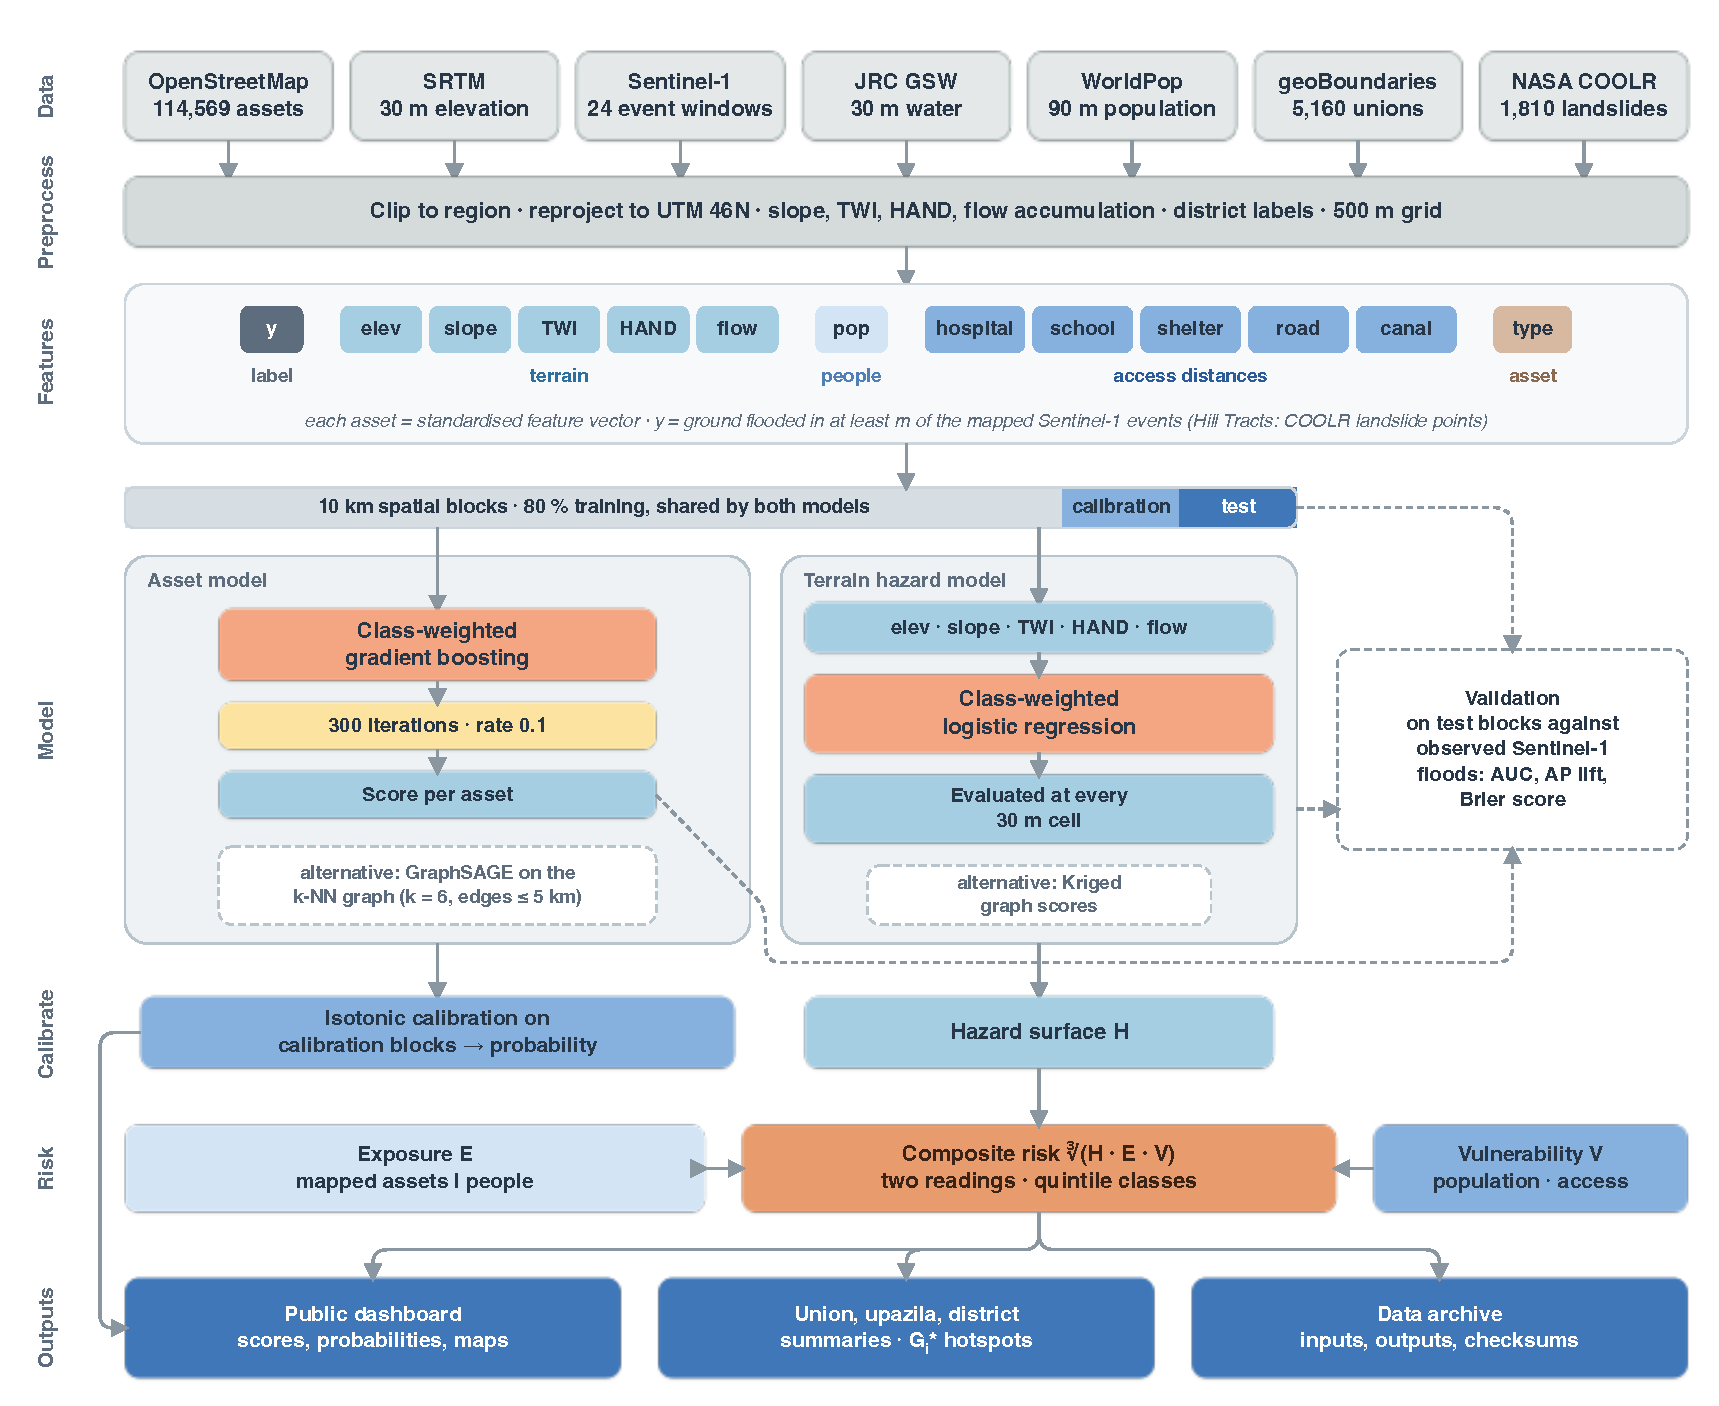
\includegraphics[width=\textwidth,height=0.72\textheight,keepaspectratio]{figures/fig_chain_national.pdf}
\caption{The processing chain, top to bottom, with the counts of the national run. Each asset enters the models as a vector of terrain, population, access-distance and asset-type features, with a label from the Sentinel-1 flood frequency. Every model trains on the same spatial blocks, and dashed connectors mark what the validation scores on the test blocks. In the landslide region a model fitted to a mapped inventory takes the place of the flood labels.}
\label{fig:chain}
\end{figure}

A region is defined by a YAML file that states only what differs from a shared base configuration and names that base with an \texttt{extends} key. The base holds the model settings, weights and thresholds, so a change to any of them reaches every region and results stay comparable. A region file carries its extent, either a bounding box or a list of districts, together with a country code, a projected coordinate system, data directories and, for validation, the flood events to map from radar, each with the dates of its window and the report those dates came from. A region defined by districts keeps only the assets, grid cells and validation points inside them, so the regions of a national partition never count the same asset twice.

The public site is the web application, which serves the outputs from an SQLite database and PMTiles vector tiles through a FastAPI service and a MapLibre GL client, so that every asset of every region is drawn at once and panning and filtering happen in the browser (Fig.~\ref{fig:dashboard}). The build step also places every asset in its union, upazila, district and division, and sums each region's results up that hierarchy, so the map shows one administrative level at a time, chosen by zoom, and a click or a cascade of pickers narrows the assets and counters to one area. The official return-period scenarios of the government's Multi-hazard Risk and Vulnerability Assessment can be laid under the assets, drawn live from the server that publishes them, and the address of the page records the view, so a copied link or a downloaded image reproduces it. A Streamlit dashboard that reads the outputs directly remains for local use. Neither front end computes anything, and every value a visitor sees can therefore be traced to a file the pipeline wrote.

\subsection{Software functionalities}

The data stages listed in Table~\ref{tab:stages} read OpenStreetMap assets either from the Overpass API, in tiles that are cached and split when the server cannot answer, or from a national extract converted once into an indexed file. Assets are clipped to the region and to the country, so that an extent crossing a land border keeps only the home side. Slope, the topographic wetness index, height above nearest drainage and flow accumulation come from 30\,m SRTM elevation, population from WorldPop, and administrative units from geoBoundaries, with divisions dissolved from their districts. The Sentinel-1 stage maps each configured event in Google Earth Engine by change detection against a dry-season baseline, following the UN-SPIDER practice \citep{unspider}, and splits a download the service refuses into quarters. It removes permanent water with the JRC surface-water record \citep{pekel2016}, and averages the event masks into a flood-frequency layer that becomes the training label.

\begin{table*}[t]
\centering
\small
\begin{tabularx}{\textwidth}{@{}l>{\raggedright\arraybackslash}X@{}}
\toprule
Stage & What it does \\
\midrule
\texttt{download}, \texttt{ingest} & fetch assets, elevation, population, boundaries and surface water, and clip them to the region \\
\texttt{clip} & drop assets across a land border from an asset file fetched earlier \\
\texttt{preprocess} & derive terrain rasters and write both label sources, radar-observed and terrain-threshold \\
\texttt{sentinel1} & map each configured flood event from radar and build the flood-frequency layer \\
\texttt{features}, \texttt{graph} & sample features at every asset and assign assets to 10\,km spatial blocks \\
\texttt{train} & fit the configured asset model on training blocks and calibrate it on calibration blocks \\
\texttt{krige}, \texttt{risk} & build the terrain and Kriged hazard surfaces, exposure, vulnerability and composite risk, and summarise them by administrative unit \\
\texttt{landslide} & fit a landslide susceptibility model to a mapped inventory \\
\texttt{validate}, \texttt{crosscheck} & score models and surfaces against observed floods, and radar masks against an independent flood database \\
\texttt{benchmark}, \texttt{sensitivity} & compare models and label sources over repeated block assignments, run the temporal hold-out, and perturb the risk weights \\
\texttt{run} & run the whole chain for one region \\
\bottomrule
\end{tabularx}
\caption{Pipeline stages, each a subcommand of the command-line interface.}
\label{tab:stages}
\end{table*}

The asset model is set in the configuration, with class-weighted gradient boosting as the default and a random forest, logistic regression and a two-layer GraphSAGE network \citep{hamilton2017} on a $k$-nearest-neighbour graph of assets available as alternatives. Scores are calibrated by isotonic regression \citep{zadrozny2002} fitted on blocks the model never trained on, with each calibration level shrunk towards the middle in proportion to how few points it holds, so that a level of three flooded points cannot return a certainty. Two hazard surfaces are written, a logistic model of each grid cell's own terrain and an ordinary Kriging of the asset scores, and the composite risk uses the one the configuration names. Composite risk is the geometric mean of hazard, exposure and vulnerability on a 500\,m grid, the aggregation the INFORM index uses \citep{inform2017}, and it is written twice, once for mapped infrastructure and once for population, with hotspots located by the Getis--Ord $G_i^*$ statistic \citep{getis1992}. For the landslide region the pipeline fits a logistic model to a mapped inventory, drawing background points only from the ground the inventory covers so that the model learns terrain rather than the mapping footprint \citep{barbetmassin2012}.

The validation suite is what distinguishes the system from a mapping tool. Every model is scored on 10\,km blocks held out from training, and the \texttt{benchmark} stage refits it over \RRBenchSeeds{} block assignments so that each difference is reported with its spread. On identical features, assets and blocks, the same stage compares the configured models with one another and with the wetness index alone, compares training on radar labels with training on terrain-threshold labels, and trains on earlier floods to score against the latest year. The \texttt{crosscheck} stage compares the radar masks with the MODIS-based Global Flood Database \citep{tellman2021}, and the \texttt{sensitivity} stage recomputes the composite under alternative and randomly perturbed weights.

\subsection{Safeguards against silent failure}

A geospatial pipeline can fail without raising an error, as when a raster stored in a projected system is sampled with longitude and latitude and returns its nodata value everywhere, leaving a model to train on constant features and labels of a single class. The pipeline therefore stops on inputs of that kind, halting if any feature comes out constant, if the labels hold a single class, if a radar event returns no imagery, or if a zonal summary overlaps no unit. Units without mapped assets are left unscored instead of scored zero, and a missing output is reported as missing.

Each of these checks, and the clipping of every region to the country, is guarded by a test in a suite of 159, which also fails if the dashboard shows mock data or random values. No figure in the documentation is typed by hand, because a build script reads each region's outputs and writes one LaTeX macro per value. A value the pipeline has not produced renders as a visible marker, and a test checks that every macro used in the documentation exists. Rerunning the pipeline and rebuilding a document therefore updates its text and its results together.

%% ─────────────────────────────────────────────────────────────────────
\section{Illustrative examples}

The pipeline was developed on three bounding-box regions, Rangpur and Rajshahi for riverine flooding, Sylhet for flash flooding and the south-west coast for cyclone surge, and then pointed at the whole country. The national partition assigns each of the \NatDistricts{} lowland districts to one of \NatRegions{} regions by flood regime, and each region needed only a configuration file listing its districts and its flood events, every event checked against a situation report and against Sentinel-1 coverage of its window before the run. The same commands scored \NatAssets{} mapped assets (Fig.~\ref{fig:national}), and the web build placed them in the national administrative hierarchy (Fig.~\ref{fig:dashboard}).

\begin{figure}[!htbp]
\centering
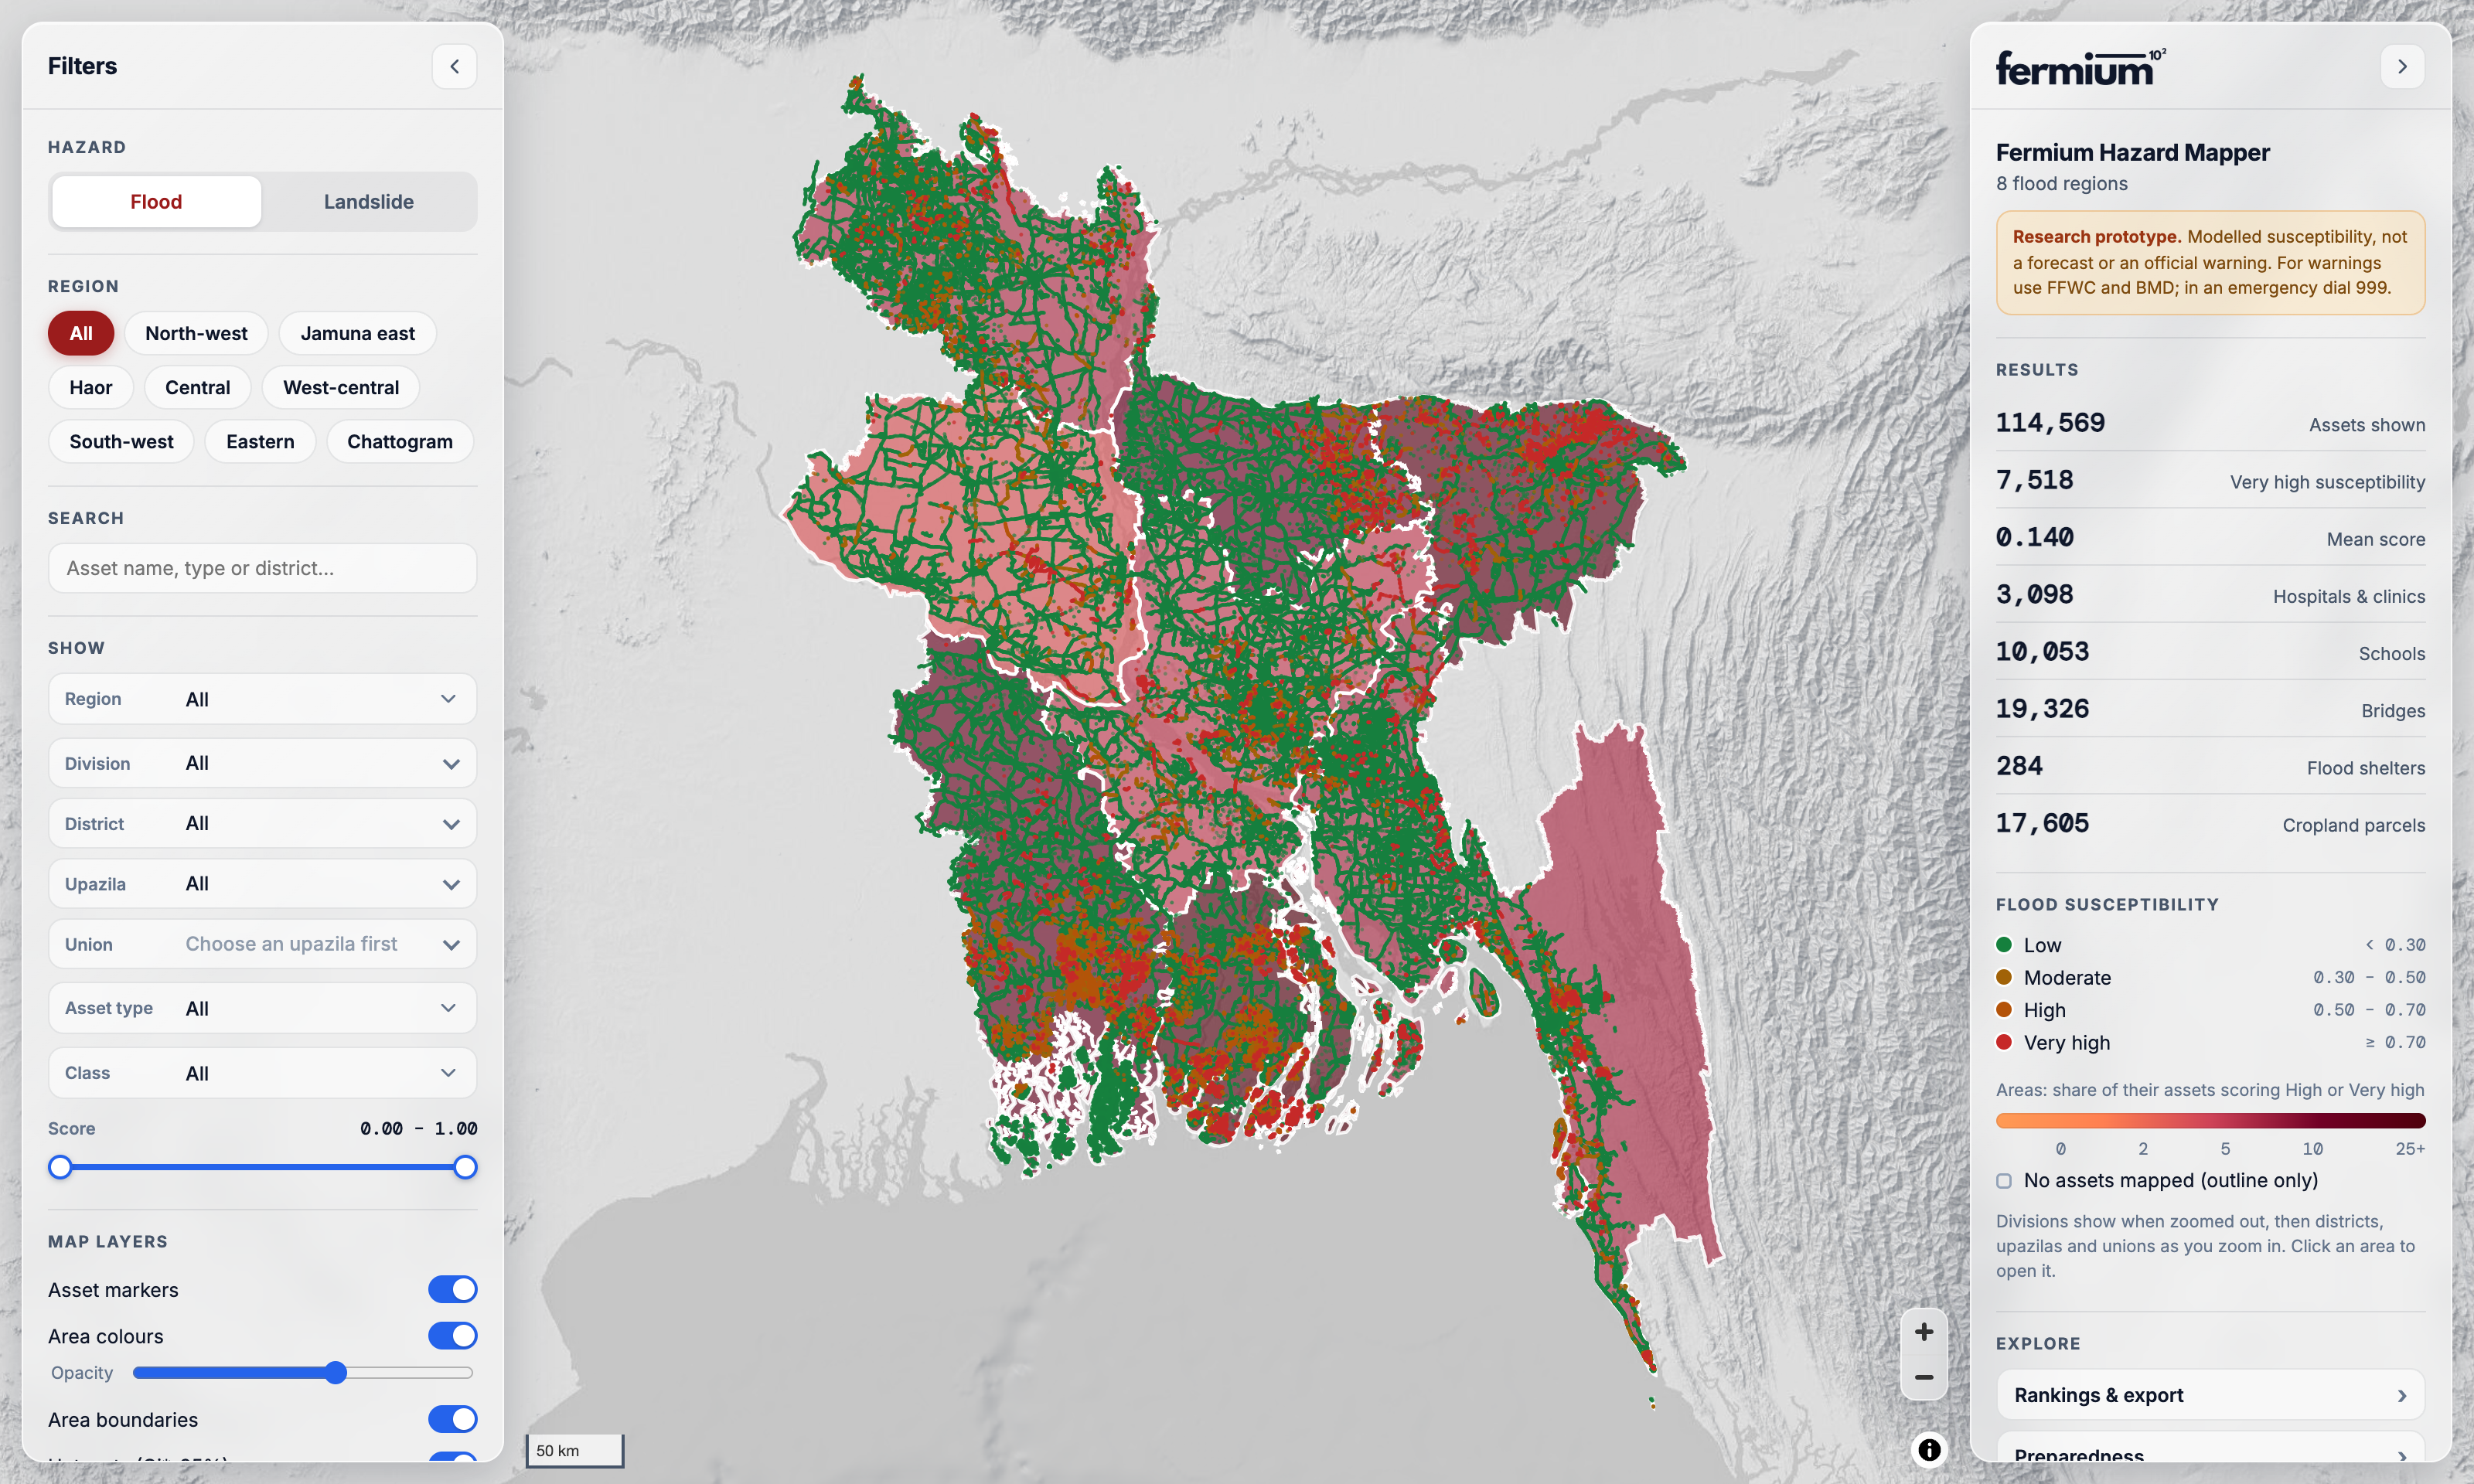
\includegraphics[width=\textwidth]{figures/fig_dashboard.png}
\caption{The web application in its national flood view. Asset markers are coloured by modelled susceptibility class and divisions by the share of their assets in the High or Very high class; zooming in replaces divisions with districts, upazilas and unions. Filters, administrative pickers and layers sit on the left; counters for whatever the filters leave visible, the legend and the model figures sit on the right.}
\label{fig:dashboard}
\end{figure}

\begin{figure}[t]
\centering
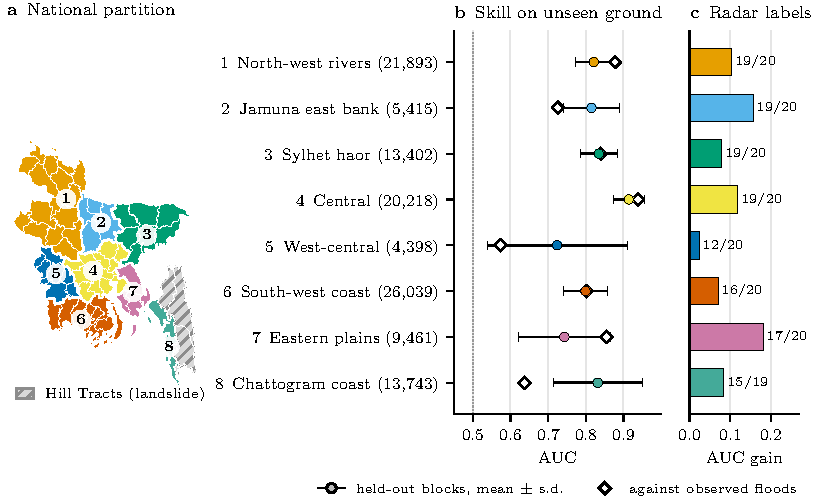
\includegraphics[width=\textwidth]{figures/fig_national.pdf}
\caption{The national partition. (a) The \NatRegions{} flood regions, numbered as in (b) and (c), and the Hill Tracts landslide region. (b) AUC of the gradient-boosted model on held-out 10\,km blocks, as mean and standard deviation over 20 block assignments, and on the held-out blocks of one assignment scored against observed floods; mapped assets in brackets. (c) AUC won by training on radar-observed flooding instead of terrain-threshold labels, with the number of assignments in which radar labels came out ahead.}
\label{fig:national}
\end{figure}

The figure carries the evidence a user needs before trusting a region. Training on radar-observed flooding beats training on terrain thresholds in every region, though in West-central only by a margin within noise. The graph network the system was first built around trails the best ordinary model in every region, by \NatGraphGapMin{} to \NatGraphGapMax{} in AUC, which is why gradient boosting is the default, and the comparison stays in the pipeline so that a future model has to beat it on the same blocks.

The temporal test compares the model with the flood record itself. In the riverine validation regions, a model trained only on floods up to 2022 ranks the ground the 2024 floods reached at \RRTempAUC{} and \SylhetTempAUC{}, and the radar record of earlier flooding ranks it at \RRTempPastAUC{} and \SylhetTempPastAUC{}.

%% ─────────────────────────────────────────────────────────────────────
\section{Impact}

Flood susceptibility studies for Bangladesh report AUCs between 0.81 and 0.984 from random splits of their own points (Section~\ref{sec:motivation}), a design that scores a model mostly beside its training data and gives one number without a spread. The software replaces that number with a validation design in which every comparison runs on the same 10\,km blocks held out from training, repeated over \RRBenchSeeds{} block assignments and reported with its spread, so a claim about a model or a data source becomes a figure that another group can check with one command.

That design opens questions earlier maps could not answer. Whether a model knows more than the flood record is tested by training on floods up to a cut-off year and scoring the next floods against the radar record of earlier flooding, a baseline that needs no model, and in the riverine validation regions the record ranked the 2024 floods better than the model did. Whether radar-observed floods make better training labels than terrain thresholds is tested by training the same model on both over the same blocks, and radar labels came out ahead in every region of the national partition, by margins that range from within noise in West-central to the largest in the Eastern plains (Fig.~\ref{fig:national}). Whether a new model architecture adds anything is tested by adding it as another configurable type, which places it in the same comparisons, and the graph network the system was first built around added nothing.

The software also reports measures that a susceptibility map alone does not. Each asset carries a calibrated flood probability, fitted on blocks the model never trained on, beside its ranking score. Each administrative unit from the union to the division is scored by the share of its mapped assets in the High or Very high class, summed over every flood region, so a division spanning several regions is scored from all of them and a unit without mapped assets is reported as missing rather than as safe. Composite risk is written once for infrastructure and once for people, so the two readings of exposure can be set side by side. These figures are served openly at \url{https://fermium.systems/hazmapper} for the whole country, beside the official scenario maps.

Reproducibility is built into the software rather than promised. No number in its documentation is typed by hand, one command reruns a validation region from the data archive without Earth Engine and checks every headline figure against it, and the pipeline stops on constant features, labels of a single class or radar events without imagery instead of publishing their results. The pipeline is not tied to Bangladesh's regions, since a new region needs only a configuration file with a bounding box or a list of districts, a country code, a projected coordinate system and a list of flood events with their dates. All inputs other than the Sentinel-1 stage come from global open datasets, that stage needs only a noncommercial Earth Engine project, and the event lists and asset weights that remain specific to Bangladesh are set in configuration files, not in the code. The input data and outputs of the three validation regions and the landslide region are archived with checksums and licences \citep{hasan2026data}.

%% ─────────────────────────────────────────────────────────────────────
\section{Limitations}

The validation the software runs also marks what its results cannot support. Where a radar record of past floods exists, it ranked the next riverine floods better than the model, so the maps complement that record rather than replace it. The terrain hazard surface is close to chance on the south-west coast, at \CoastalSurfaceTerrainObsAUC{} across the grid, and near or below chance wherever embankments, tides or flash floods decide where water lies, as on the Jamuna east bank, because terrain does not describe them. Regions with few mapped floods give unstable scores: West-central, whose two waterlogging events were documented only in newspapers, varies widely between block assignments and is marked as low-data on the dashboard. The landslide model, at an AUC of \CHTLSAUC{} from \CHTLandslides{} landslides mapped after a single storm, describes where that storm triggered failures rather than susceptibility to landslides in general.

Two further limits sit in the inputs rather than the models. Exposure depends on OpenStreetMap, whose completeness varies widely \citep{herfort2023} and has not been measured for rural Bangladesh, so composite risk describes mapped exposure. Vulnerability uses population density and three access distances and leaves out income, housing and age structure. The dashboard states each of these limits beside the map it qualifies.

%% ─────────────────────────────────────────────────────────────────────
\section{Conclusions}

Fermium Hazard Mapper joins radar-observed flood labels, spatially blocked validation and a public dashboard in one open and reproducible chain, now covering the whole of Bangladesh. Its main contribution is a validation suite that runs every comparison on identical held-out areas and reports it with its spread, together with a design that stops on silent errors instead of publishing their results.

The next versions follow from what the validation shows. Embankment and tide data would give the surge and flash-flood regions a hazard surface that terrain alone cannot, more mapped events would firm up low-data regions such as West-central, and retraining the landslide model on the multi-year inventory of \citet{rabby2019} would move it beyond a single storm.

%% ── Declarations ─────────────────────────────────────────────────────
% Long role names and URLs set without running into the margin.
\sloppy
\section*{CRediT authorship contribution statement}
\textbf{Md Rakib Hasan:} Conceptualization, Methodology, Software, Validation, Formal analysis, Data curation, Visualization, Writing -- original draft, Writing -- review \& editing. \textbf{Shoumik Zubyer:} Conceptualization, Writing -- review \& editing.

\section*{Declaration of competing interest}
Md Rakib Hasan is affiliated with Fermium Systems, which hosts the public dashboard. The software is released under the MIT licence and the dashboard is free to use. The authors declare no other competing interests.

\section*{Data availability}
The code is at \url{https://github.com/rakibhhridoy/rimes-mapathon}, and the release this article describes is archived at \SoftwareDOI{} \citep{hasan2026software}. Input data and outputs for the three validation regions and the landslide region are archived at \url{https://doi.org/10.5281/zenodo.23108572} \citep{hasan2026data}, and the national partition is reproduced by the configuration files in the repository. A single command, \texttt{python scripts/demo.py}, downloads a validation region's archive, reruns the pipeline on it without Earth Engine in a few minutes, and checks every headline figure against the archived outputs.

\section*{Acknowledgements}
The authors thank the Regional Integrated Multi-Hazard Early Warning System for Africa and Asia (RIMES) for organising the Mapathon in which the first version of the software competed. Infrastructure data are \copyright{} OpenStreetMap contributors, under the Open Database Licence. Population data are from WorldPop, University of Southampton, CC BY 4.0. Administrative boundaries are from geoBoundaries, William \& Mary geoLab, CC BY 4.0. Sentinel-1 data are Copernicus Sentinel data, processed in Google Earth Engine. Landslide locations are from NASA's Cooperative Open Online Landslide Repository. The scenario maps shown beside the results are the Department of Disaster Management's Multi-hazard Risk and Vulnerability Assessment, served by the United Nations Satellite Centre (UNOSAT), and the basemap relief is from Esri.

\bibliographystyle{elsarticle-num-names}
\bibliography{../references,softwarex}

\end{document}
